\documentclass[11pt,letterpaper]{article}
\usepackage[utf8]{inputenc}
\usepackage{fontspec}
\usepackage[margin=1in]{geometry}
\usepackage{graphicx}
\usepackage{pgffor}
\usepackage{amsmath}
\usepackage{amssymb}
\usepackage{fancyhdr}
\usepackage{hyperref}
\usepackage{subcaption}
\usepackage{bbm}
\usepackage{lscape}
\usepackage{ulem}

% ------------------------------------------------------

\DeclareMathOperator*{\argmin}{arg\,min}
\DeclareMathOperator*{\argmax}{arg\,max}
\DeclareMathOperator{\Var}{Var}
\DeclareMathOperator{\Cov}{Cov}
\def\inprob{\,{\buildrel p \over \longrightarrow}\,} 
\def\indist{\,{\buildrel d \over \longrightarrow}\,} 

\DeclareMathOperator\F{\mathcal{F}}

% ------------------------------------------------------
 
\usepackage{fontspec}
\usepackage[usenames,dvipsnames]{xcolor}
\usepackage{listings}

%%
%% Julia definition (c) 2014 Jubobs
%%
\lstdefinelanguage{Julia}%
  {morekeywords={abstract,break,case,catch,const,continue,do,else,elseif,%
      end,export,false,for,function,immutable,import,importall,if,in,%
      macro,module,otherwise,quote,return,switch,true,try,type,typealias,%
      using,while,%
      exit,whos,edit,load,is,isa,isequal,typeof,tuple,ntuple,uid,hash,finalizer,convert,promote,
      subtype,typemin,typemax,realmin,realmax,sizeof,eps,promote_type,method_exists,applicable,
      invoke,dlopen,dlsym,system,error,throw,assert,new,Inf,Nan,pi,im,begin,while,for,in,return,
      break,continue,macro,quote,let,if,elseif,else,try,catch,end,bitstype,ccall,do,using,module,
      import,export,importall,baremodule,immutable,local,global,const,Bool,Int,Int8,Int16,Int32,
      Int64,Uint,Uint8,Uint16,Uint32,Uint64,Float32,Float64,Complex64,Complex128,Any,Nothing,None,
      function,type,typealias,abstract},%
   sensitive=true,%
   alsoother={$}, % $
   morecomment=[l]\#,%
   morecomment=[n]{\#=}{=\#},%
   morestring=[s]{"}{"},%
   morestring=[m]{'}{'},%
}[keywords,comments,strings]%

\lstset{%
    language         = Julia,
    basicstyle       = \scriptsize\ttfamily,
    keywordstyle     = \bfseries\color{blue},
    stringstyle      = \color{magenta},
    commentstyle     = \color{ForestGreen},
    numberstyle      = \color{Gray},
    showstringspaces = false,
	showtabs         = false,
	upquote          = false,
    breaklines       = true,
    extendedchars    = true,
}

\begingroup
  \catcode0=12 %
  \makeatletter
  \g@addto@macro\lst@DefEC{%
    \lst@CCECUse\lst@ProcessLetter
   αβγδεϵζηθϑγκλμνξπϖρϱσςτυϕφχψωΓΔΘΛΞΠΣΥΦΨΩ∇% *** add Unicode characters ***
    ^^00% end marker
  }%
\endgroup

\setmonofont{Consolas}

% ------------------------------------------------------

\graphicspath{{../plots/pdf/}{../plots/}}
\setlength\parindent{0.0in}

% ------------------------------------------------------

\title{\textbf{Homework 7} \\ Labor Economics}
\author{Mark Agerton and Nick Frazier}
\date{Due Mon, Feb 23}

% ------------------------------------------------------

\begin{document}

\maketitle

\section{Setup}
Wages are
\begin{align*}
y_0 &= \delta_0 + \beta_0 x + \theta + \epsilon_0 \\
y_1 &= \delta_1 + \beta_1 x + \alpha_1\theta + \epsilon_1
\end{align*}
Also define the utility shifter function $C$ and an index function $I$
\begin{align*}
C &= \gamma_0 + \gamma_2 z + \gamma_3 x + \alpha_C \theta  \\
I &= E[y_1 - y_0 - C|\F]  \\
  &= \underbrace{(\delta_1 - \delta_0 - \gamma_0)}_{\widetilde \delta} + \underbrace{(\beta_1 - \beta_0 - \gamma_3)}_{\widetilde \beta} x_i - \gamma_2 z + \underbrace{(\alpha_1 - 1- \alpha_C)}_{\widetilde \alpha} \theta - \epsilon_{c}
\end{align*}
The distribution of shocks is
\[
\left. \begin{pmatrix} \epsilon_{i,0} \\ \epsilon_{i,1} \\ \epsilon_{i,C} \end{pmatrix} \right|_{x_i,z_i,\theta_i}
\sim N
\left[ \begin{pmatrix} 0 \\ 0 \\ 0 \end{pmatrix}, \begin{pmatrix} \sigma_0^2& 0 & 0\\0& \sigma_1^2& 0 \\0 & 0& \sigma_C^2\end{pmatrix}	\right] 
\]
The information set for the agent is $\F$. The preference shock $\epsilon_C \in \F$, but $\{\epsilon_0,\epsilon_1\} \notin \F$. The decision rule is
\[
s = 1 \Longleftrightarrow E[I \geq 0 | \F]
\]

\section{Q1}
There is no unobserved heterogeneity in this model since we know $\theta$. Thus,
\[
E\left[ \begin{matrix} y_{0} \\ y_{1} \end{matrix} \middle | x_i,\theta_i, s=k \right]
=
\begin{bmatrix} 
	\delta_0 + x\beta_0 + \theta         \\  
	\delta_1 + x\beta_1 + \alpha_1\theta 
\end{bmatrix} + 
\underbrace{E\left[ \begin{matrix} \epsilon_{0} \\ \epsilon_{1} \end{matrix} \middle | x_i,\theta_i, \epsilon_c:big/small \right]}_{0}
\]
This is straight-up OLS, which means we recover $\{\delta, \beta, \alpha_1, \sigma^2_0, \sigma^2_1\}$. 
\begin{align*}
\Pr[S=1|\F] 
&= \Pr\left[\epsilon_c \leq \widetilde \delta + \widetilde \beta x - \gamma_2 z + \widetilde \alpha \theta \middle | \F\right] \\
&= \Phi\left[\frac{\overbrace{\left[(\delta_1 - \delta_0) + (\beta_1-\beta_0)x + (\alpha_1 - 1)\theta\right]}^{\text{known number}} -\gamma_0 - \gamma_2 z - \gamma_3 x - \alpha_c \theta }{\sigma_c} \middle | \F\right]
\end{align*}
Now we can get $\left\{ \gamma_0, \gamma_2, \gamma_3, \alpha_c, \sigma_c^2 \right\}$


\section{Q2}

Now we don't know $\theta$ but agents do. However, we do have two measurement equations $m \in \{A,B\}$:
\begin{align*}
M_{iA} &= x_i^M \beta_A^M + \theta_i + \epsilon_{iA}^M \\
M_{iB} &= x_i^M \beta_B^M + \alpha_B\theta_i + \epsilon_{iB}^M
\end{align*}
where $\epsilon_m^M \sim N(0,\sigma^{M2}_m)$ are i.i.d. 

\subsection{Heckman two-step}

We can write
\begin{align*}
E[y_1 | x,z,s=1] 
&= \delta_1 + \beta_1 x + E[\epsilon_1 + \alpha_1\theta | x,z, I\geq 0] \\
&= \delta_1 + \beta_1 x + \alpha_1 E[\theta | x,z, I\geq 0] \\
&= \delta_1 + \beta_1 x + \alpha_1\sigma^* E\left[\frac{\theta}{\sigma^*} \middle|0 \leq \widetilde \delta + \widetilde \beta x - \gamma_2 z + \underbrace{(\alpha_1 - \alpha_0 - \alpha_c)\theta - \epsilon_c}_\eta  \right] \\
&= \delta_1 + \beta_1 x + \alpha_1\sigma^* E\left[\frac{\theta}{\sigma^*} \middle| \eta \geq - \left( \widetilde \delta + \widetilde \beta x - \gamma_2 z  \right) \right]
\end{align*}
Define $\eta \equiv (\alpha_1 - \alpha_0 - \alpha_c)\theta - \epsilon_c$. Then 
\[
\begin{pmatrix} \eta \\ \theta \end{pmatrix} 
\sim N
\left[ 
	\begin{pmatrix} 0 \\ 0  \end{pmatrix}, 
	\begin{pmatrix} 
		\sigma^{*2}     & (\alpha_1 - \alpha_0 - \alpha_c)\sigma^2_\theta \\
		(\alpha_1 - \alpha_0 - \alpha_c)\sigma^2_\theta & \sigma^2_\theta \\
	\end{pmatrix}
\right] 
\]
where $\sigma^{*2} = (\alpha_1 - \alpha_0 - \alpha_c)^2\sigma^2_\theta + \sigma^2_c$. We can project $\theta$ onto $\eta$, which means
\[
\theta = \frac{\Cov(\eta,\theta)}{\Var \eta } \eta + \nu = \frac{(\alpha_1 - \alpha_0 - \alpha_c)\sigma^2_\theta}{\sigma^{*2}}\eta + \nu
\]
where
\[
\nu \sim N\left( 0, \sigma^2_\theta \left( 1- \rho_{\eta\theta}^2\right)\right)
\qquad\text{and} \qquad
\rho_{\eta\theta} = \frac{(\alpha_1 - \alpha_0 - \alpha_c)\sigma^2_\theta}{\sigma^{*}\sigma_\theta}
\]

\subsubsection{Step 1}

We know that $S=1 \Leftrightarrow \eta \geq -(\widetilde \delta + \widetilde \beta X - \widetilde \gamma Z) + \eta \geq 0$. So, in the first step of the procedure, we estimate
\begin{align*}
\Pr[S=1|\F] 
&= 1 - \Phi\left[\overbrace{\frac{\delta_1  - \delta_0 - \gamma_0}{\sigma^*}}^{\widetilde \delta} + \overbrace{\frac{\beta_1 - \beta_0 - \gamma_3}{\sigma^*}}^{\widetilde \beta} X - \overbrace{\frac{\gamma_2}{\sigma^*}}^{\widetilde \gamma} Z 
\right] \\
&= 1- \Phi\left[\widetilde \delta + \widetilde \beta X - \widetilde\gamma_2 Z 
\right] 
\end{align*}
This gives us $\left\{ \widetilde \delta, \widetilde \beta, \widetilde \gamma \right\}$.

\subsection{Step 2}

Letting $t \equiv -(\widetilde \delta + \widetilde \beta X - \widetilde \gamma Z)$, we can now write
\begin{align*}
E[y_0 | x,z,s=1] 
&= \delta_0 + \beta_0 x + \alpha_0 \frac{(\alpha_1 - \alpha_0 - \alpha_c)\sigma^2_\theta}{\sigma^*} \overbrace{\frac{-\phi(t)}{\Phi(t)}}^{\lambda_0} \\
&= \delta_0 + \beta_0 x + \alpha_0 \left( \rho_{\eta\theta}\sigma_\theta \right) \lambda_{0i} \\
E[y_1 | x,z,s=1] 
&= \delta_1 + \beta_1 x + \alpha_1 \frac{(\alpha_1 - \alpha_0 - \alpha_c)\sigma^2_\theta}{\sigma^*} \underbrace{\frac{\phi(t)}{1-\Phi(t)}}_{\lambda_1} \\
&= \delta_1 + \beta_1 x + \alpha_1 \left( \rho_{\eta\theta}\sigma_\theta \right) \lambda_{1i} \\
\end{align*}

This gives us estimates for $\left\{ \delta_0, \delta_1, \beta_0, \beta_1, (\alpha_0\rho_{\eta\zeta}\sigma_\theta), (\alpha_1\rho_{\eta\zeta}\sigma_\theta) \right\}$

\subsection{Step 3}

Now we can use the covariances. We have
\begin{align*}
\Cov(Y_0 - \delta_0 - \beta_0 X,\; M^A - \beta_A X^M) &= \Cov(Y_0, M^A | X, X^M, Z) &= \alpha_0 \sigma^2_\theta \\
\Cov(Y_0 - \delta_0 - \beta_0 X,\; M^B - \beta_B X^M) &= \Cov(Y_0, M^B | X, X^M, Z) &= \alpha_0 \alpha_B \sigma^2_\theta \\
\Cov(Y_1 - \delta_1 - \beta_1 X,\; M^A - \beta_A X^M) &= \Cov(Y_1, M^A | X, X^M, Z) &= \alpha_1 \sigma^2_\theta \\
\Cov(Y_1 - \delta_1 - \beta_1 X,\; M^B - \beta_B X^M) &= \Cov(Y_1, M^B | X, X^M, Z) &= \alpha_1 \alpha_B \sigma^2_\theta \\
\Cov(M^A - \beta_A X^M         ,\; M^B - \beta_B X^M) &= \Cov(M^A, M^B | X^M      ) &= \alpha_B \sigma^2_\theta
\end{align*}
We use these covariances to identify the rest of the model. 
\begin{align*}
\widehat{\alpha_0 / \alpha_1} &= (\alpha_0\rho\sigma^2_\theta)/(\alpha_0\rho\sigma^2_\theta) \\
\widehat \alpha_B &= \Cov(Y_0, M^B)/\Cov(Y_0, M^A)  \\
\widehat \sigma^2_\theta &= \Cov(M^A, M^B)/\widehat \alpha_B  \\
\widehat \alpha_0 &= \Cov(Y_0, M^A)/ \widehat\sigma_\theta^2  \\
\widehat \alpha_1 &= \Cov(Y_1, M^B)/ \widehat\sigma_\theta^2  \\
\widehat \sigma^2_A &= \Var(M^A) - \widehat\sigma^2_\theta  \\
\widehat \sigma^2_B  &= \Var(M^B) - \widehat \alpha_B^2 \widehat \sigma^2_\theta  \\
\widehat \rho &= \widehat{ \alpha_0 (\rho\sigma_\theta)} / (\widehat \alpha_0 \sqrt{\widehat \sigma_\theta^2})  \\
              &= \widehat{ \alpha_1 (\rho\sigma_\theta)} / (\widehat \alpha_1 \sqrt{\widehat \sigma_\theta^2})  \\
\widehat \sigma_0^2 &= \Var(Y_0) - \widehat{ \alpha_0 (\rho\sigma_\theta)}^2\left[ 1 - t\widehat \lambda_0 + \widehat \lambda_0^2 \right] - \widehat \sigma^2_\theta(1-\widehat \rho^2) \\
\widehat \sigma_1^2 &= \Var(Y_1) - \widehat{ \alpha_1 (\rho\sigma_\theta)}^2\left[ 1 - t\widehat \lambda_1 + \widehat \lambda_1^2 \right] - \widehat \sigma^2_\theta(1-\widehat \rho^2) \\
\widehat \alpha_c &= \left\{ \alpha_c \in R \middle | (\widehat \rho \widehat \sigma_\theta) - (\widehat \alpha_1 - \widehat \alpha_0 - \alpha_c)\widehat \sigma^2_\theta \left[(\widehat \alpha_1 - \widehat \alpha_0 - \alpha_c)^2 \widehat \sigma_\theta^2 + 1 \right]^{-1/2} =0 \right\} \\
\widehat \gamma_0 &= \left( \widehat \delta_1 -\widehat \delta_0 \right) - \widehat{\widetilde{\delta}} \times \widehat{\sigma^*} \\
\widehat \gamma_3 &= \left( \widehat \beta_1 - \widehat\beta_0 \right) - \widehat{\widetilde{\beta}} \times \widehat {\sigma^*} \\
\widehat \gamma_2 &= \widehat{\widetilde \gamma}\times \widehat{\sigma^*}
\end{align*}

%
%A probit first-step has given us $\left\{ (\delta_1 - \delta_0 -\gamma_0)/\sigma_c, (\beta_1 - \beta_0 - \gamma_3)\sigma_c), \gamma_2/\sigma_c \right\}$. With the second step, we now get $\{\delta_1, \delta_0, \beta_1, \beta_0\}$ and the ratio $\alpha_1/\alpha_0$. \sout{We can back out $\{\gamma_0/\sigma_c, \gamma_2/\sigma_c, \gamma_3/\sigma_c\}$ from the original probit equations. We also get the quantity $(\alpha_1 - \alpha_0 - \alpha_c)\sigma^2_\theta$ since we have $\sigma_c^2$.} However, we have 3 $\alpha$s and only 2 equations for them, so those aren't identified. \textbf{If we normalized $\alpha_c = 1$, then we would identify $\gamma$s for sure... but not clear if we need to do this.} We can now turn to variances and covariances. Recall
%\[
%\rho_{\eta\theta}\sigma_\theta = \frac{(\alpha_1 - \alpha_0 - \alpha_c)\sigma^2_\theta}{\sqrt{(\alpha_1 - \alpha_0 - \alpha_c)^2\sigma^2_\theta + \sigma^2_c}}
%\]
%It is clear to see that these are of little help since we have a bunch of parameters in the euqations for the variances: 
%\begin{align*}
%\Var (Y_0| \eta  <  -t ) 
%	&= \alpha_0^2 \Var\left(\theta\middle| \eta <    t\right) + \sigma^2_0  \\
%	&= \alpha_0^2 \left( \rho_{\eta\theta}\sigma_\theta \right)^2 \left[1 - t \lambda_0 - \lambda_0^2 \right] + \sigma^2_\theta \left( 1- \rho_{\eta\theta}^2\right) + \sigma^2_0\\
%%	&= \alpha_0^2 \frac{(\alpha_1 - \alpha_0 - \alpha_c)\sigma^2_\theta}{\sqrt{(\alpha_1 - \alpha_0 - \alpha_c)^2\sigma_\theta^2 + \sigma_0^2}} + \sigma_\theta^2 \left(1 - \frac{(\alpha_1 - \alpha_0 - \alpha_c)^2\sigma^4_\theta}{\sigma_0^2 \left[(\alpha_1 - \alpha_0 - \alpha_c)^2\sigma_\theta^2 + \sigma_0^2 \right]} \right) \\
%\Var (Y_1| \eta\geq -t ) &= \alpha_1^2 \Var\left(\theta\middle| \eta \geq t\right) + \sigma^2_1 
%\end{align*}
%Fortunately, with the measurement equations, we can say things. Recall $I=E[Y_1 - Y_0 - C|X,Z,\theta]$. If we had an estimate of $I$, we would be in business... and when we do EM/MLE, we do get an estimate of $I$ (right). \textbf{Previously: ``I have no idea what to do with the last 2 eqns b/c how do we compute $I$ w/ out $\theta$ This is maybe why we need MLE and EM??''}
%\begin{align}
%\Cov(Y_0 - \beta_0 X, M^A - X^M\beta_A) &= \alpha_0 \sigma^2_\theta \\
%\Cov(Y_0 - \beta_0 X, M^B - X^M\beta_B) &= \alpha_0 \alpha_B \sigma^2_\theta \\
%\Cov(Y_1 - \beta_1 X, M^A - X^M\beta_A) &= \alpha_1 \sigma^2_\theta \\
%\Cov(Y_1 - \beta_1 X, M^B - X^M\beta_B) &= \alpha_1 \alpha_B \sigma^2_\theta \\
%\Cov\left[I - \widetilde \delta - \widetilde \beta x -\gamma_2 z,\; \left(M^A - X^M\beta_A \right)\right]
%	&= (\alpha_1 - \alpha_0 - \alpha_c) \sigma^2_\theta \\
%\Cov\left[I - \widetilde \delta - \widetilde \beta x -\gamma_2 z,\; \left(M^B - X^M\beta_B \right)\right]
%	&= (\alpha_1 - \alpha_0 - \alpha_c) \alpha_B \sigma^2_\theta \\
%\Cov\left[I - \widetilde \delta - \widetilde \beta x -\gamma_2 z,\; \left(Y_0 - X\beta_0 \right)\right] 
%	&= (\alpha_1 - \alpha_0 - \alpha_c) \alpha_0\sigma^2_\theta \\
%\Cov\left[I - \widetilde \delta - \widetilde \beta x -\gamma_2 z,\; \left(Y_1 - X\beta_1 \right)\right] 
%	&= (\alpha_1 - \alpha_0 - \alpha_c) \alpha_1 \sigma^2_\theta
%\end{align}
%The top four equations give us two measurements for $\alpha_B$. The bottom four plus knowledge of $(\alpha_1 - \alpha_0 - \alpha_c)\sigma^2_\theta$ from the two-step gives us $\alpha_0$ and $\alpha_1$ (just divide them). With $\alpha_k$s in hand plus $\alpha_B$ give us multiple measurements for $\sigma^2_\theta$. We plug these in to the variances for $\Var(Y_k|X,Z,s=k)$ and get $\sigma_k^2$. Done.

\subsection{MLE approach}

The contribution to the likelihood of any given individual $i$ is now the product of the likelihood of the wage and choice times the product of the likelihoods of the test equations.
\begin{align*}
L_i &= 
	         \left[f(y_{1i}|X,\theta,s_i=1)\Pr(s_i=1|X,Z,\theta)\right]^{s_i} \\
	& \times \left[f(y_{0i}|X,\theta,s_i=0)\Pr(s_i=0|X,Z,\theta)\right]^{1-s_i} \\
	& \times f(m^A_i|X_i^M,\theta) \\
	& \times f(m^B_i|X_i^M,\theta) \\
	& \times f(\theta)
\end{align*}
Define $q_i \equiv 2s_i - 1$. Since we only observe $y_{1i}$ or $y_{i0}$, we simply use $y_i$ in the likelihood equation. We can log everything and integrate w/ respect to $\theta$. 
\begin{align*}
\mathcal L_i 
	&= \int_\theta \log \left[1 - \Phi\left(
		q_i \times \frac{(\delta_1 - \delta_0 - \gamma_0) + (\beta_1 - \beta_0 - \gamma_3)X_i - \gamma_2 Z_i + (\alpha_1 - \alpha_0 - \alpha_c)\theta}{\sigma_c} 
		\right) \right] \\
	&+    s_i  \log\left[\phi\left( \frac{y_i - \delta_1 - \beta_1 x_i - \alpha_1 \theta}{\sigma_1} \right) \right] \\
	&+ (1-s_i) \log\left[\phi\left( \frac{y_i - \delta_0 - \beta_0 x_i - \alpha_0 \theta}{\sigma_0} \right) \right] \\
	&+ \log\left[\phi\left(\frac{M_i^A - X^M_i\beta_A - \theta        }{\sigma_A} \right)\right] \\
	&+ \log\left[\phi\left(\frac{M_i^B - X^M_i\beta_B - \alpha_B\theta}{\sigma_B} \right)\right] \\
	&+ \log\left[\phi\left(\frac{\theta}{\sigma_\theta}\right)\right] d\theta
\end{align*}


We maximize the $\sum_{i=1}^N \sum_{j=1}^J w_j \mathcal L_i(\theta_j) \phi\left(\frac{\theta_j}{\sigma_\theta}\right)$. To update $\sigma_\theta$, we do
\[
(\sigma_\theta^2)^{(t)} =\Var\left( \frac{(\widehat Y_i - Y_i) + (\widehat M_i^A - M_i^A) + (\widehat M_i^B - M_i^B)}{3} \right)
\]

\section{Q4}

We lose equations 1, 2 and 7. Additionally, we are more likely to observe one side of the distribution of $\theta$ now since agents select on $\theta$. Thus, we need to include a control function in our measurement equations and the analogous component of the likelihood equation. If we do this, we still have identification because we can use 
\[
\frac{\Cov\left[I - \widetilde \delta - \widetilde \beta x -\gamma_2 z,\; \left(Y_1 - X\beta_1 \right)\right]}
{\Cov\left[I - \widetilde \delta - \widetilde \beta x -\gamma_2 z,\; \left(M^A - X^M\beta_A \right)\right]} = \alpha_1
\]
Ta-da!


\begin{figure}[h]
	\centering
	\begin{subfigure}[b]{0.3\textwidth}\centering 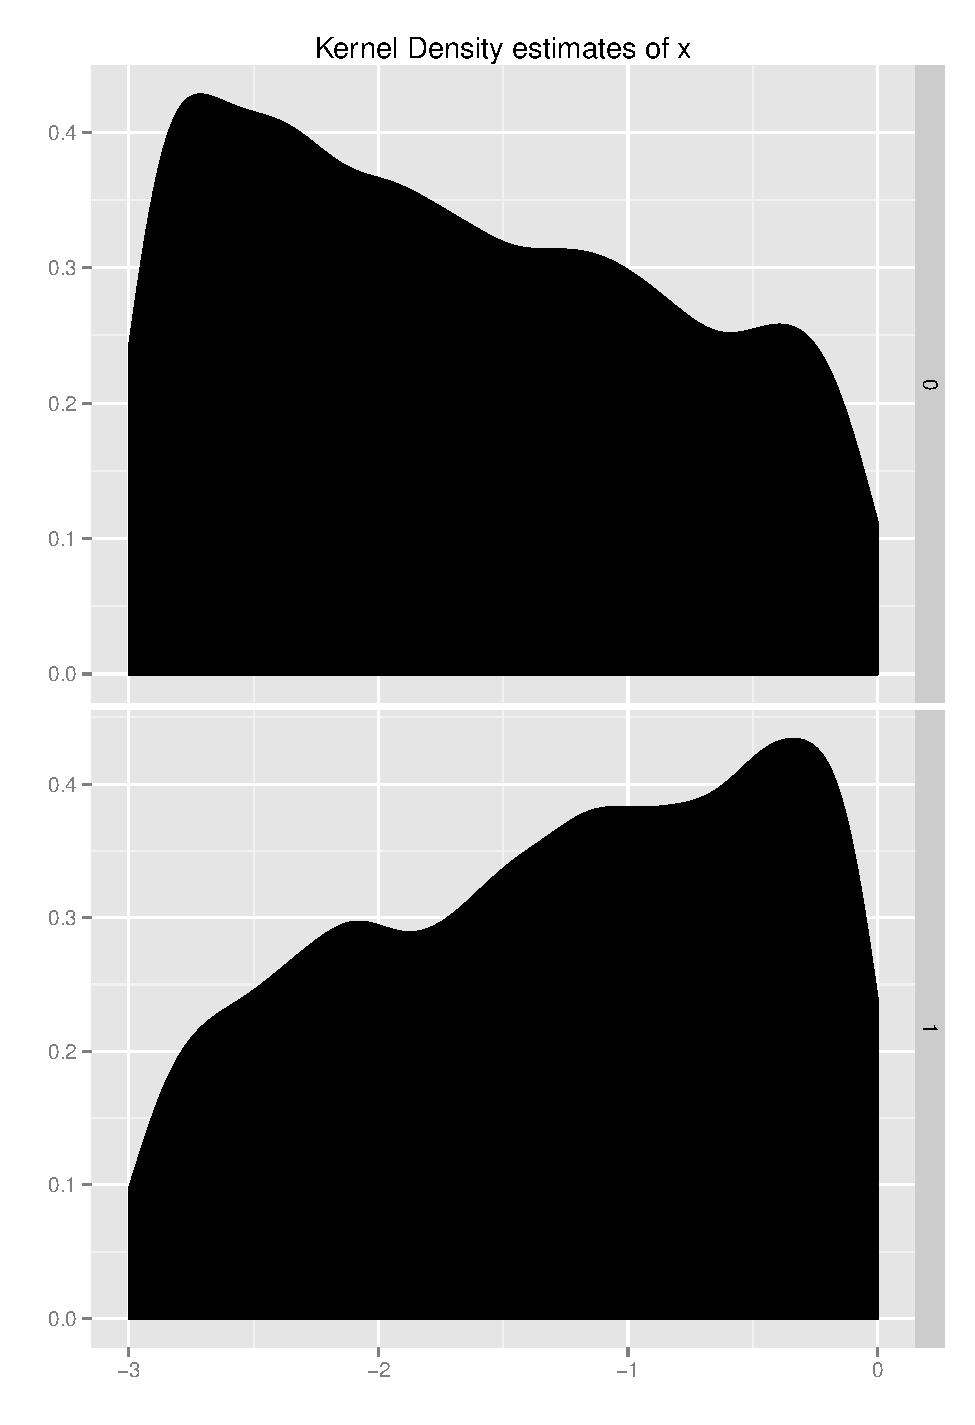
\includegraphics[width=1\textwidth]{x}  \end{subfigure}
	\begin{subfigure}[b]{0.3\textwidth}\centering 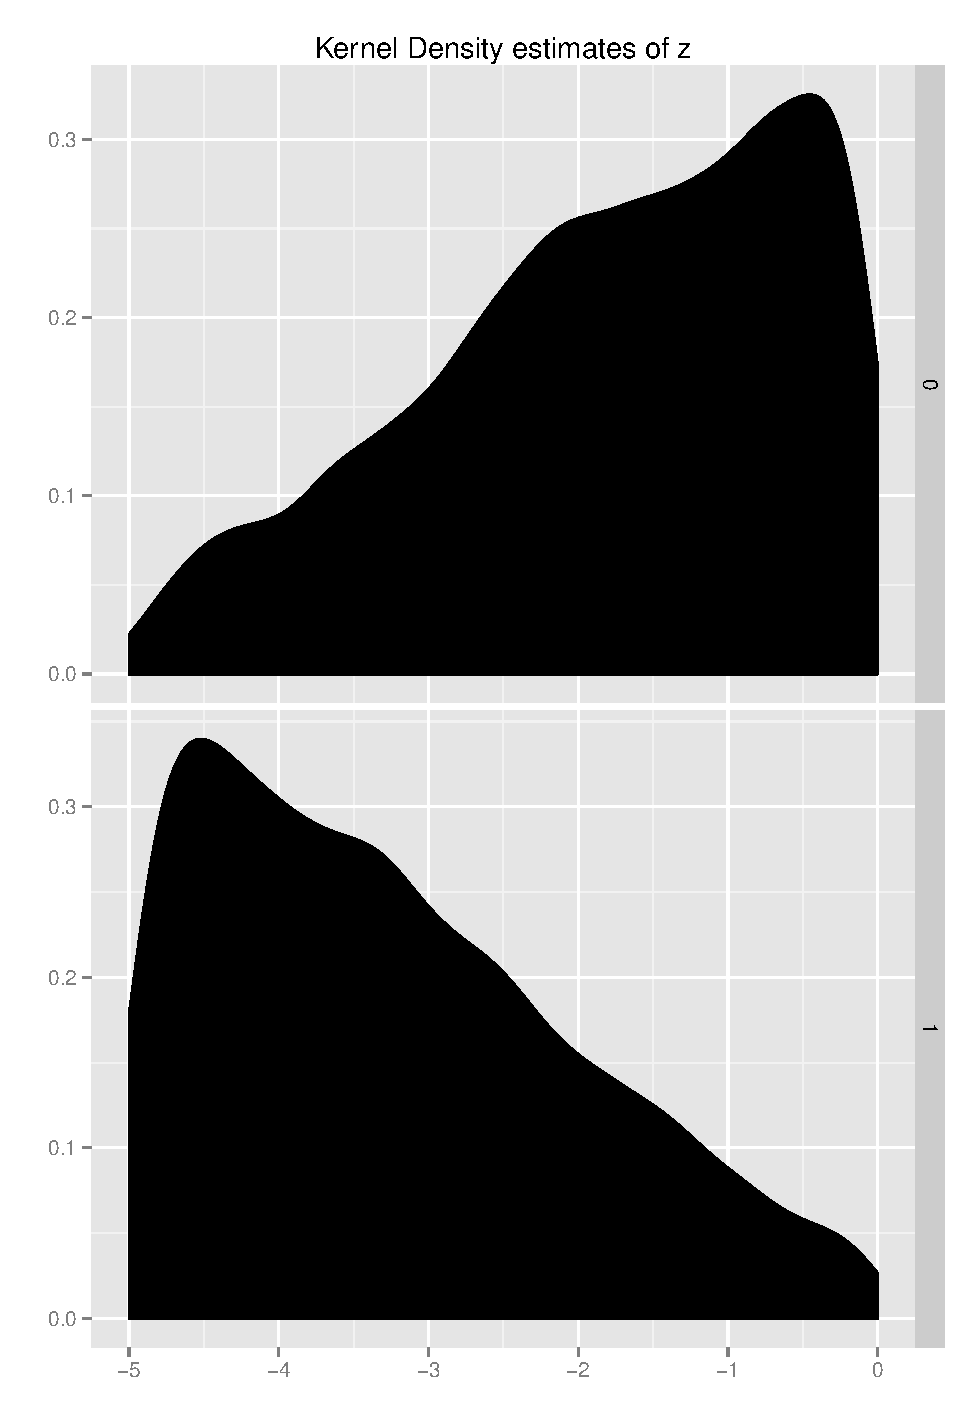
\includegraphics[width=1\textwidth]{z}  \end{subfigure}
    \begin{subfigure}[b]{0.3\textwidth}\centering 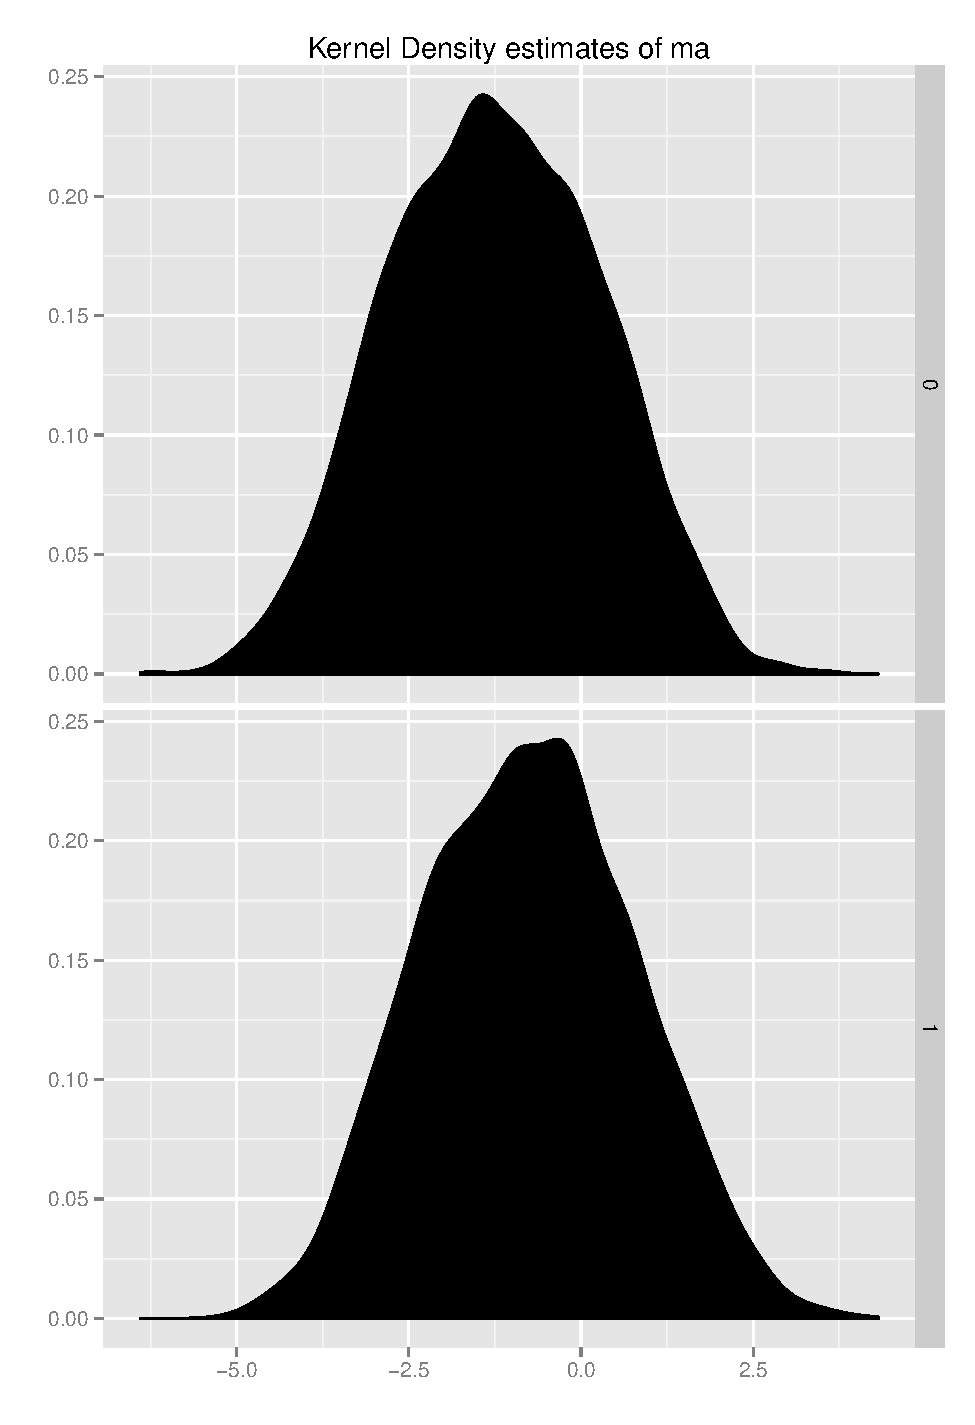
\includegraphics[width=1\textwidth]{ma} \end{subfigure}

    \begin{subfigure}[b]{0.3\textwidth}\centering 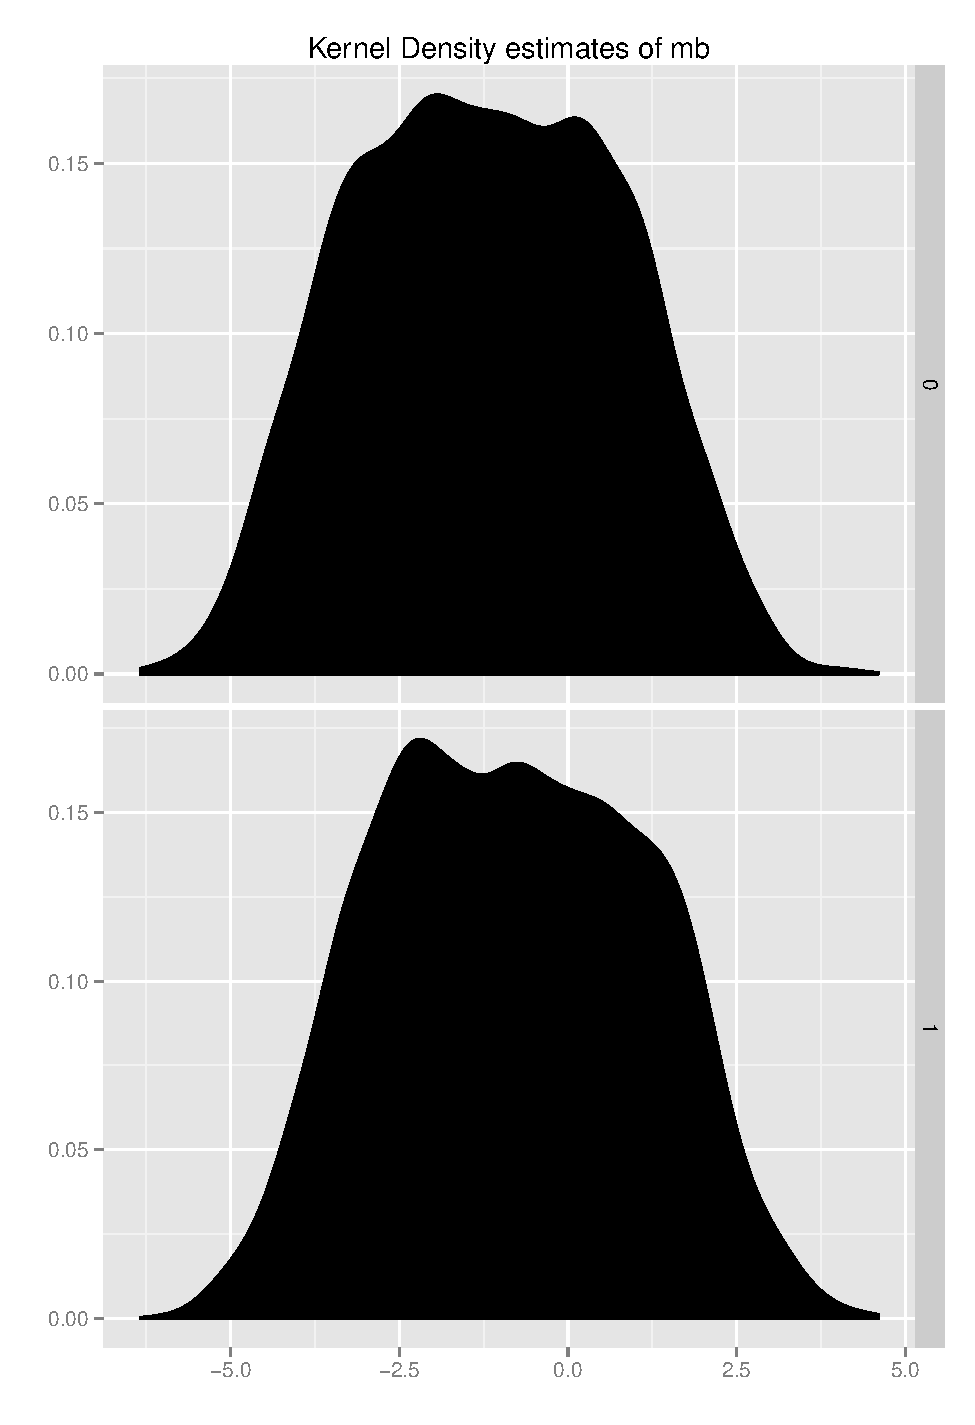
\includegraphics[width=1\textwidth]{mb} \end{subfigure}
    \begin{subfigure}[b]{0.3\textwidth}\centering 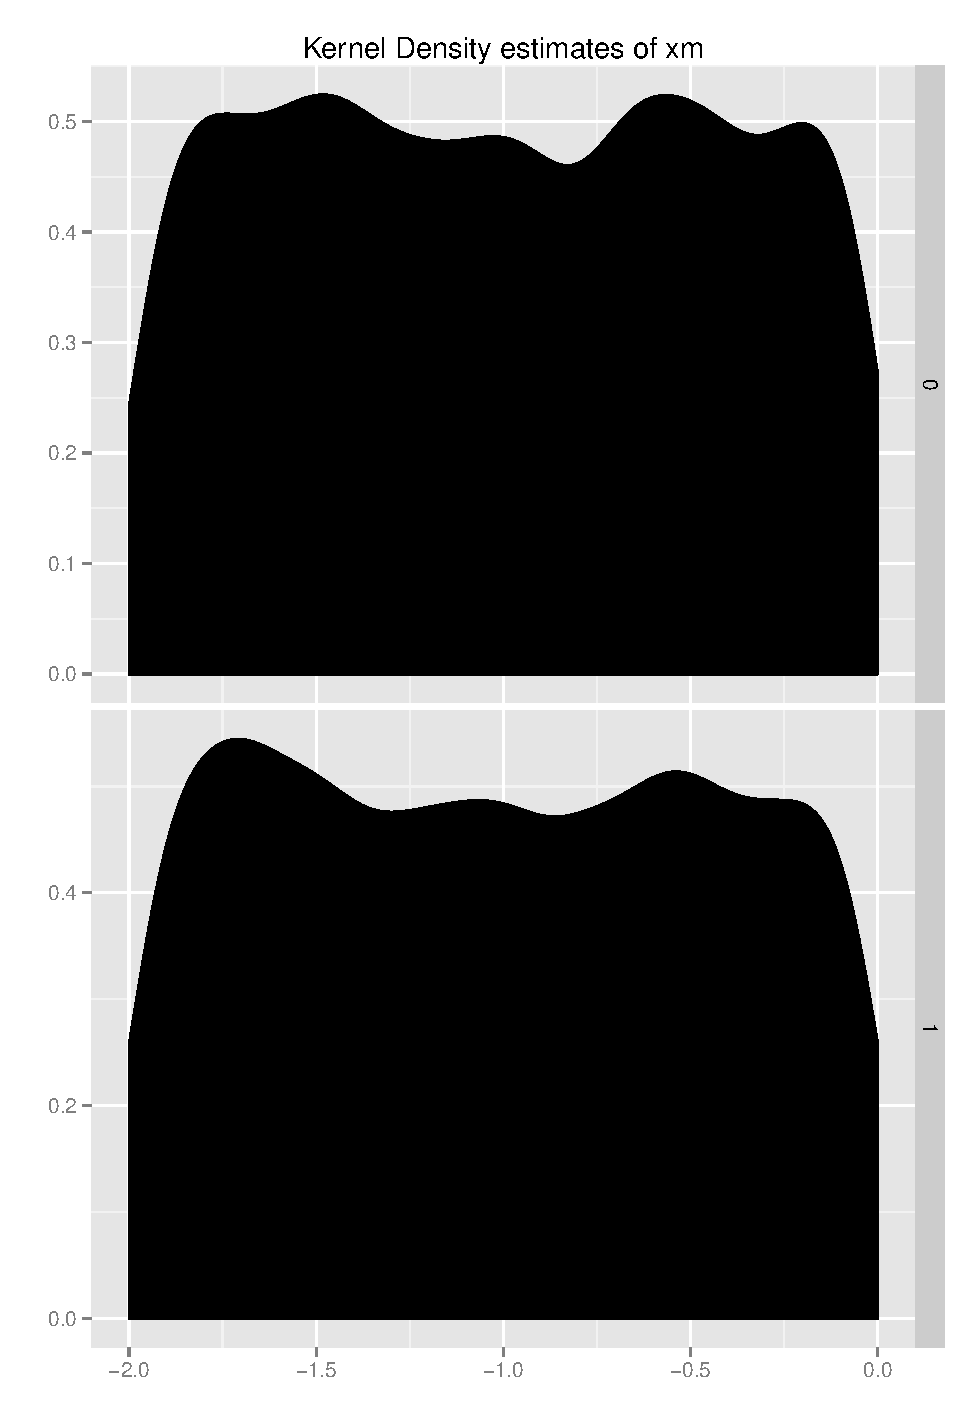
\includegraphics[width=1\textwidth]{xm} \end{subfigure}
    \begin{subfigure}[b]{0.3\textwidth}\centering 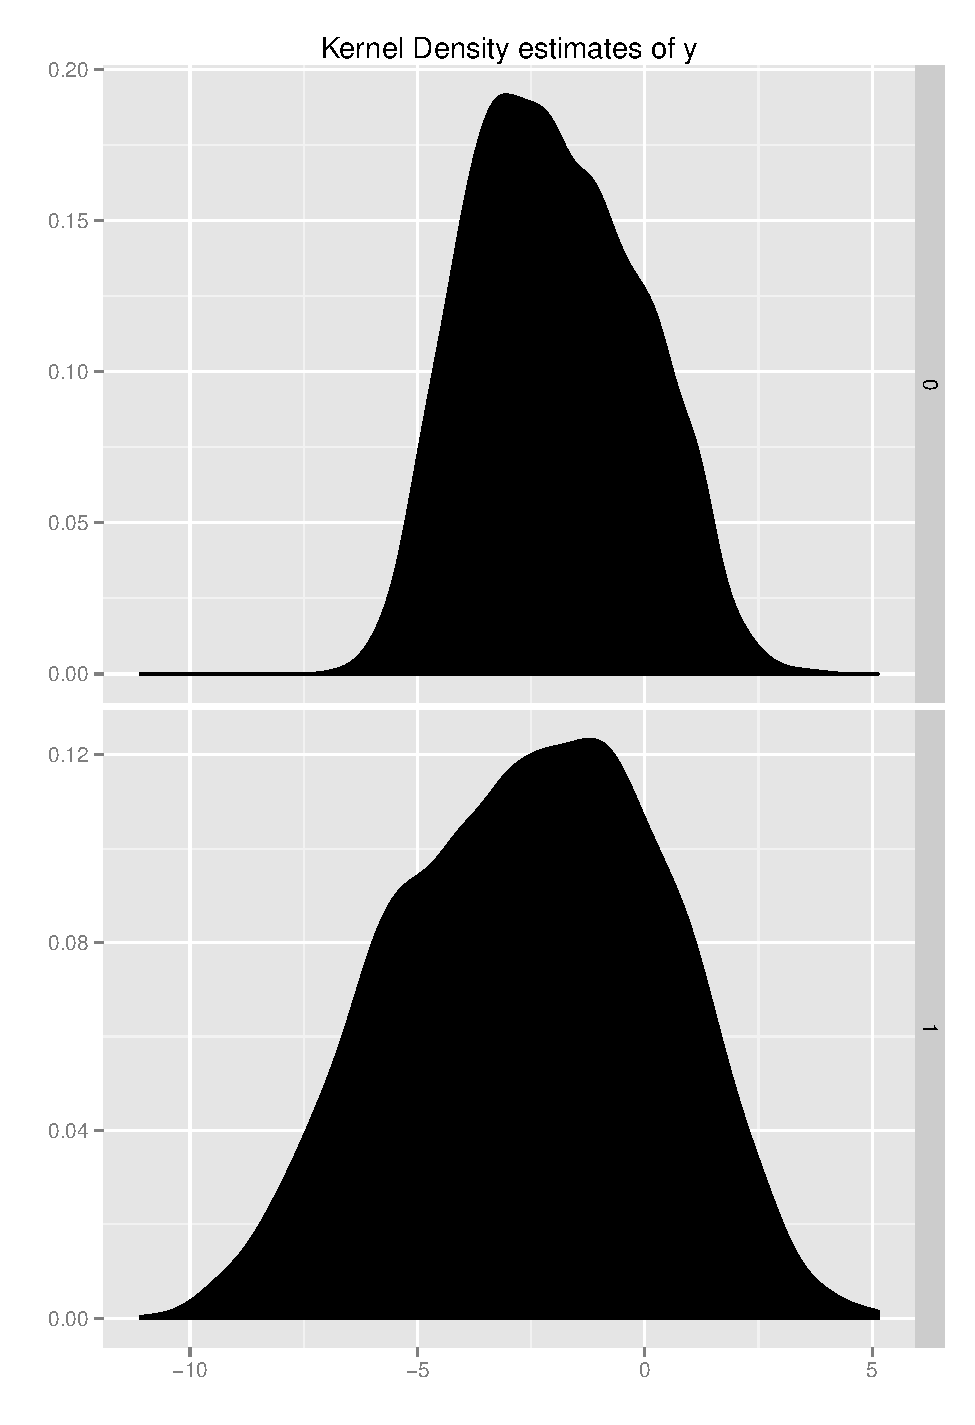
\includegraphics[width=1\textwidth]{y} \end{subfigure}    
    \caption{Histograms}		
\end{figure}	



\clearpage
\section{Results}
\lstinputlisting[frame=single,language={},caption=Results]{../Hwk7-Results.txt}

\section{Main call}
\lstinputlisting[frame=single, caption=Main call]{../code/main.jl}

\section{Functions and weights}
\lstinputlisting[frame=single, caption=Functions used]{../code/functions.jl}
\lstinputlisting[frame=single, caption=Quadrature weights (from MATLAB)]{../code/HG_wts.jl}



\end{document}
